
%(BEGIN_QUESTION)
% Copyright 2003, Tony R. Kuphaldt, released under the Creative Commons Attribution License (v 1.0)
% This means you may do almost anything with this work of mine, so long as you give me proper credit

The following ladder logic diagram (for a steam heater control) contains a serious mistake:

$$\includegraphics[width=15.5cm]{i02322x01.eps}$$

This is a mistake I've seen many students make.  Explain what the mistake is, and draw a corrected version of this relay circuit.

\vskip 20pt \vbox{\hrule \hbox{\strut \vrule{} {\bf Suggestions for Socratic discussion} \vrule} \hrule}

\begin{itemize}
\item{} Why do you suppose this is a common mistake for students to make when sketching a ladder logic diagram?  Despite it being in error, there is a certain logic to it.
\item{} If a real circuit were wired in this manner, what would it do?  How would it behave?
\item{} If a real circuit were wired in this manner, how could you diagnose the nature of the problem using a multimeter?
\end{itemize}

\underbar{file i02322}
%(END_QUESTION)





%(BEGIN_ANSWER)

Never, ever connect load devices in series in a control circuit such as this!

%(END_ANSWER)





%(BEGIN_NOTES)

Discuss with your students why load devices are never to be connected in series.  What would be the effect of doing so?  Have them answer this question in terms of normal operation, and also in terms of operation given a failure condition in one of the series-connected load devices.
 
%INDEX% Relay, diagram: ladder logic

%(END_NOTES)


